\section{Summary}
This section is comprised of brief descriptions of each chapter present in this dissertation.
\subsection{Methodology}
This section is an overview of the various methodologies we used in the development of this project. This includes our Research, Development and Testing methodologies as well as how they were implemented throughout the development life-cycle. It also gives a brief overview of certain technologies that were used to match these methodologies.

\subsection{Tech Review}
This chapter contains a description of the various technologies and tools we used in the development of this project. These include tools for Project Management, Application Development and Front end, Cloud and Server side tools, Containerize Software, Testing and the various Software Development Kit's and libraries used. 

\subsection{System Design}
This chapter discusses the components and their technologies in greater detail. As well as how they are implemented into the System as a whole and the design decisions made during the development.

\subsection{System Evaluation}
This chapter is an evaluation of the initial project objectives and compares them to the final implementation of the project. We also reflect over the project as a whole, including the limitations and what can be improved.

\subsection{Conclusion}
A brief overview of the implemented project and reflection of the development process as well as our thoughts and what we learned.

\section{Web Applications}
A Web Application is an application that is invoked in a web browser while accessing the Internet. Web Applications come in a wide variety of types from small-scale application that are short lived to long-term and large-scale applications that are distributed across multiple servers. Applications that utilize a HTML front-end have the benefit of universal cross-platform access. This eliminates compatibility issues as all users have access to the same version. \cite{hadley2006web} HTTP protocols are used to fetch these HTML document resources. Other languages such as Javascript and CSS can be used to provide further implementation and styling options that are lacking in a HTML.

\section{Goals and Objectives}
Our main goal was to develop a web application hosted on a remote virtual machine that would allow the users to share ideas, information and help organize and manage their games.

\subsection{Technical Objectives}
\begin{itemize}
    \item Store Character and User information on a secure server
    \item Allow users to Post and Reply to a Forum
    \item A Messaging system and Friends list between users
    \item Create private groups between users
    \item Help users find a group or individual
    \item Create Characters
\end{itemize}

\section{Work Allocation and Planning}
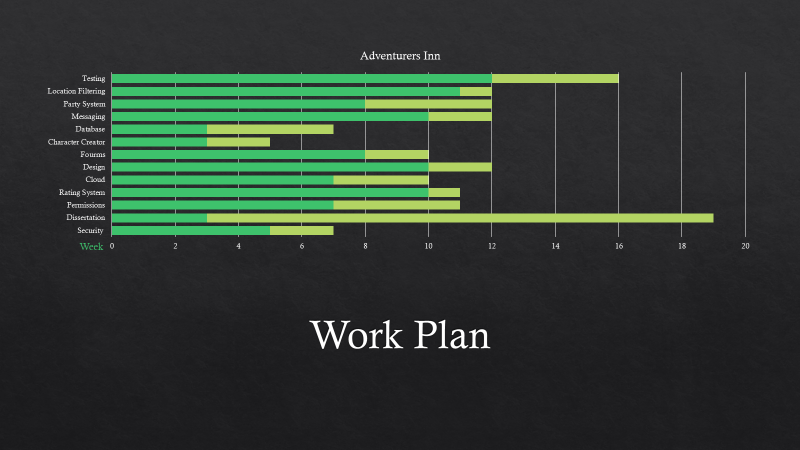
\includegraphics[scale=0.8]{./img/WorkPlanOrginal.png}
We have recorded our work incrementally in the journal page on Github the work we individually did, including what was not found in commits such as changes to the Firebase Cloud Firestore, where rules can be altered for the server. As well we have documented problems we faced and the rationale behind the decisions we made as well as the rational behind them. Included in this is our original plan from the first semester.

\subsection{Work Plan}
\subsubsection{Front End}
\begin{itemize}
    \item Initial research on Angular: Antaine and Colin  
    \item Basic Create Character: Antaine  
    \item Advanced Create Character: Colin
    \item Bootstrap and Styling of Application: Colin  
    \item Forums: Antaine
    \item Navigation: Colin
    \item Messaging: Antaine 
    \item Add Username: Colin
    \item Profile: Antaine and Colin
\end{itemize}
\subsubsection{Back End}
\begin{itemize}
    \item Initial Research on Databases(NOSQL vs SQL): Antaine  
    \item Firebase Database Creation: Antaine   
    \item Create, Read, Update and Delete functionality: Antaine
    \item Database Implementation: Antaine
    \item Angular Routing: Antaine 
    \item Login and Registration: Colin
    \item Security and Authentication: Antaine
    \item Docker: Colin
    \item Database Design: Antaine and Colin  
\end{itemize}

\subsubsection{Cloud and Hosting}  
\begin{itemize}
  \item Initial research on Cloud Services: Colin  
  \item Azure Cloud Implementation: Colin  
  \item Connected Virtual Machine to Database: Colin  
  \end{itemize}

\subsubsection{Dissertation}
\begin{itemize}
    \item Abstract: Antaine
    \item Introduction: Antaine and Colin
    \item Methodology: Antaine
    \item Technology Review: Colin
    \item System Design: Antaine and Colin
    \item System Evaluation: Antaine and Colin
    \item Conclusion: Colin
\end{itemize}

\section{Project Objectives}
The primary goal of this project was to create a web application to be used as tool to enhance a users experience with planning, managing and playing Tabletop Role Playing Games (TTRPGS), with a focus on Dungeons and Dragons 5th edition. The user should be able to share their thoughts and ideas, questions and much more on a forum. It will allow users to share information to a group of 'Players' and Dungeon Master/Game Master, as well as allowing them to quickly reference their character information which the web app would help the user make by reducing the amount of information required to make a character and the amount of paper resources required to manage. The app should also aid the user in finding a group by posting to the forums or for a group to search for a player and include the kind of sessions they intend to run.


